\documentclass[12pt,a4paper,titlepage,twoside]{report}
\usepackage[T1]{fontenc}
\usepackage[english, spanish]{babel}
\usepackage[utf8]{inputenc}
\usepackage{lmodern}
\usepackage{graphicx}
\usepackage{csquotes}
\usepackage{xcolor}
\usepackage{url}
\usepackage[backend=biber,style=alphabetic,
sorting=ynt]{biblatex}
\addbibresource{biblio.bib}
% http://tug.ctan.org/tex-archive/macros/latex/contrib/fancyhdr/
\usepackage{fancyhdr}
\pagestyle{fancy}
\fancyhf{}
\fancyhead[LE,RO]{\nouppercase \rightmark}
\fancyhead[LO,RE]{\nouppercase \leftmark}
\fancyfoot[C]{\thepage}

%Carpeta de imagenes
\graphicspath{ {img/}}

\newcommand{\Keywords}[1]{\vfill\noindent{\small{\em Palabras clave}: #1}}
\definecolor{grisclar}{gray}{0.5}
\definecolor{grisfosc}{gray}{0.25}

% Editar con los datos correspondientes
\newcommand{\titulo}{Diseño e implementación de un Cluster de virtualización en alta disponibilidad para los servicios de emergencias del Consorcio Provincial de Bomberos de Valencia}
\newcommand{\titulacion}{Ingeniería en Informática}
\newcommand{\autor}{María Alexandra Hermosilla Semikina}
\newcommand{\director}{J. Alberto Conejero}

\title{\titulo}
\author{\autor}

\begin{document}
% Portada basada en el ejemplo de:
% http://en.wikibooks.org/wiki/LaTeX/Title_Creation

\begin{titlepage}
\begin{center}

% Logos UPV y ETSINF
\begin{minipage}{0.49\linewidth}
\begin{flushleft}

\includegraphics[height=1.5cm]{./logo-upv}
\end{flushleft}
\end{minipage}
\begin{minipage}{0.49\linewidth}
\begin{flushright}

\includegraphics[height=1.5cm]{./logo-etsinf}
\end{flushright}
\end{minipage}

\vspace{2cm}

\begin{color}{grisfosc}
\large
Escola Tècnica Superior d'Enginyeria Informàtica\\[0.2cm]
Universitat Politècnica de València\\[1.9cm]
\end{color}

% Título del proyecto y titulación
{\LARGE \bfseries \titulo}\\[1.5cm]
\textsc{\large Proyecto Final de Carrera}\\[0.4cm]
\textcolor{grisclar}{\large\titulacion}\\[5.0cm]

% Autor, director y fecha
\begin{flushright} \large
\emph{Autor:} \autor\\[0.4cm]
\emph{Director:} \director\\[0.6cm]
\today
\end{flushright}

%\vfill
% Bottom of the page
%{\large \today}

\end{center}

\end{titlepage}


\begin{abstract}
Este proyecto nació a partir de la necesidad de un cluster de virtualización que estuviera en alta disponibilidad para albergar las herramientas que utiliza el Consorcio Provincial de Bomberos de Valencia tanto para los servicios de emergencia como los servicios internos. 
El Consorcio Provincial de Bomberos de Valencia ha ido aumentando los servicios que presta a nivel interno como a nivel operativo en los servicios de emergencia, consecuentemente es necesario ampliar su infraestructura de virtualización como adaptarse al nuevo hardware que se ha incorporado a la infraestructura ya existente.
Para ello, se ha construido un cluster de virtualización basado en tecnologías como Xen, corosync y pacemaker.

\Keywords{Virtualización, HA, Alta disponibilidad, Xen, Servicios de emergencia, Cluster, Debian, Linux,Corosync, Pacemaker, ocfs2, Máquina Virtual,GNU}
\end{abstract}

\tableofcontents

\chapter{Introducción}

En octubre de 2012 accedí al Consorcio Provincial de Bomberos de Valencia como becaria para realizar las labores de apoyo en las áreas de administración de sistemas y helpdesk. Los primeros meses de la beca se me formó en las tecnologías usadas en la infraestructura utilizada para dar servicio a la sede central y a los diferentes parques que forman el Consorcio. Posteriormente y ante la urgencia de desplegar nuevos servicios, se me asignó al proyecto de la creación de un nuevo cluster de virtualización sobre el hardware Unified Computing System (UCS) de Cisco con cuatro blades listos para la instalación y configuración del cluster.
\par Debido a la proximidad de la puesta en marcha de los nuevos servicios se dio máxima prioridad a este proyecto ya que el cluster existente no disponía de los recursos necesarios para albergar todos los servicios. Por lo tanto, este cluster se convierte en el nuevo núcleo central de esta infraestructura crítica. 
\par
Una infraestructura crítica se define como aquella que es necesaria para proporcionar los servicios esenciales. Si estas infraestructuras sufren una caída por cualquier motivo puede suponer una fuente de perturbaciones graves en materia de seguridad. Por ello, este proyecto tiene una delicadeza importante, ya que no solo dará soporte a las actividades diarias del Consorcio, si no que sustenta las herramientas para el servicio de extinción y prevención de incendios.
\par
En este documento repasaremos el contexto en el cual se desarrolla este proyecto, como también algunos conceptos básicos de lo que es la virtualización y cómo funciona. Con estos conocimientos se podrá entender porqué se ha escogido la opción implementada.
\par
A lo largo del capítulo 2, veremos qué es el Consorcio Provincial de Bomberos de Valencia y como funciona. Además veremos cual era la infraestructura de virtualización anterior y qué servicios se prestaban hasta ese momento tanto hacia el ciudadano como también hacia el usuario interno. Veremos también los nuevos servicios que se prestarán desde el nuevo cluster. Para finalizar este capítulo veremos los requisitos del cluster que se han establecido y que junto a los criterios de selección nos permitieron seleccionar la opción más adecuada.
\par 
En el capítulo 3 revisaremos los criterios de selección y los diferentes soluciones que se habían barajado durante la fase de análisis. Muchas de las soluciones no se han tenido en cuenta, y por lo tanto, no aparecen entre las seleccionadas porque no cumplían con los requisitos definidos en el capítulo anterior.
\par
En el capítulo 4, veremos de forma detallada cómo se ha realizado la implementación de la solución seleccionada. Se ha dividido en varias secciones, las cuales se corresponden a las diferentes etapas que se han seguido. Esto permitirá una mejor comprensión de la implementación y de cómo funciona la solución.

Para finalizar, analizaremos la solución implementada para verificar que cumple con las funciones definidas para este proyecto. También expondremos las ventajas y desventajas de esta solución. 




\chapter{Antecedentes}

En la administración de sistemas siempre ha habido una gran problemática alrededor de la optimización de los recurso. Estos recursos no solo son a nivel de hardware, si no que también a nivel de refrigeración, consumo eléctrico y espacio, entre otros factores. El coste del mantenimiento era extremadamente elevado para entidades que disponían de infraestructuras informáticas muy grandes, ya que no solo era necesario disponer de repuestos, si no también de un elevado número de personal dedicado a esta labor.
\par
Desde la llegada de la virtualización, la informática ha sufrido una gran revolución en este aspecto. La virtualización consiste en una capa de software que corre en un sistema operativo que crea una abstracción entre el hardware y el software a ejecutar. Para este software, esta capa, es totalmente transparente, ya que ve los mismos recursos de hardware que vería un sistema operativo nativo. El software puede ser cualquier recurso que necesitemos como una computadora, sistema operativo, dispositivo de almacenamiento, aplicaciones o redes. Esto permite que, en caso de fallo de hardware, este software se pueda trasladar a otro hardware que corra la misma capa de abstracción y el software no se percate del cambio y siga funcionando sin problemas. 
\par
Como se puede apreciar, la virtualización presente una serie de ventajas respecto a las infraestructuras físicas. De estas ventajas se puede destacar las siguientes:
\begin{itemize}
\item \textbf{Aislamiento:} Cada máquina virtual es independiente una de la otra y del hypervisor. Por lo que si una de ellas falla, no afecta a las demás como tampoco al hypervisor.
\item \textbf{Seguridad:} En caso de lograr acceso privilegiado a una de estas máquinas virtuales, sólo se obtendría acceso a dicha máquina, dejando intactas el resto de máquinas y  el hypervisor donde reside dicha máquina virtual.
\item \textbf{Flexibilidad:} Las máquinas virtuales, al ser software, se les puede asignar los recursos necesarios (CPU, RAM, HDD...) sin necesidad de comprar un hardware concreto para ellas. Esto permite ampliarlas en un momento de uso alto de recursos o quitarlos cuando no son necesarios.
\item \textbf{Agilidad:} La puesta en marcha de una máquina virtual suele ser un proceso sencillo. Se puede hacer a través de rellenar un fichero con los recursos necesarios o a través de un asistente de creación. Con ello, una máquina virtual está funcionando en cuestión de minutos.
\item \textbf{Portabilidad:} El hecho de que las máquinas virtuales sean un par de ficheros,permite cambiarla de hypervisor o hardware sin gran problema. Solo es mover unos ficheros y volver a ejecutar la máquina.
\end{itemize}
\par 
Todas estas características son las que se busca en una infraestructura donde el número de servicios prestados es alto y deben estar en alta disponibilidad. Este es el caso del Consorcio Provincial de Bomberos de Valencia. Donde el número de servicios de información prestados son elevados y diversos. Algunos de ellos es necesario que estén operativos las 24 del día. 
El Consorcio cuenta en estos momentos con un personal que asciende a más de 800 personas, entre las cuales no solo se encuentra el personal operativo, sino también de personal administrativo. Cada uno de estos dos grupos de usuarios requiere de herramientas diferentes y especializadas para su labor. 
\par
Para el personal operativo es necesario que los servicios usados para su labor estén operativos siempre y poder acceder a ellos en cualquier momento y lugar. Por una parte, el Consorcio es el responsable de recibir los servicios solicitados por parte del 112 de la Generalitat Valenciana que requieran la intervención de los bomberos. Sin embargo, esta parte esta gestionada por parte del propio 112 GVA. Para la gestión del servicio a prestar sí se usa un software propio que esta gestionado internamente. Este servicio es usado no solo por parte de los operadores, sino que también por parte de todo el personal operativo. Esto quiere decir que tiene que estar disponible desde cualquier parque de bomberos de la provincia de Valencia, incluyendo los parques de voluntarios.
\par
Por otra parte, el personal administrativo es el que más servicios requiere, ya que son los responsables de toda la gestión de la organización. Esto quiere decir, que a pesar de ser el grupo minoritario, son los que más recursos necesitan para realizar su labor.
\section{Consorcio Provincial de Bomberos de Valencia}
Durante los años 60, gracias a la expansión económica, la provincia de Valencia sufrió una gran transformación socioeconómica que conllevo a un aumento de población e industrialización. Estos factores influyeron de manera notoria en el aumento del riesgo y en la demanda de los servicios de emergencias.Por este motivo, en 1982 se constituyeron los primeros servicios de emergencias en la provincia de Valencia en forma de Consorcios Comarcales. Se agruparon en mancomunidades a varios municipios por comarcas con el objetivo de facilitar la prestación de este servicio. De esta forma, se crearon 7 consorcios comarcales con la ayuda de la Diputación de Valencia: Horta Nord, Horta Sud, Camp de Morvedre, Ribera Baixa, Ribera Alta-Valldigna, La Safor y La Costera.
\par
Esta diseminación dejó patente las carencias y problemas de organización y coordinación. Por este motivo, el 31 de octubre de 1986 se constituye un único órgano provincial, el Consorcio Provincial de Bomberos de Valencia, tras la aprobación de sus Estatutos por la Generalitat, la Diputación de Valencia y los 132 municipios que se integraron en él.
\par
Actualmente, el Consorcio cubre una superficie de 10.671,48 kilómetros cuadrados, 5.819 kilómetros cuadrados de masa forestal, más de 3.000 kilómetros de carreteras, 1.700.829 vehículos y cerca de 184.483 empresas contabilizadas en la provincia de Valencia. Como también el número de pueblos que se encuentran adheridos a esta mancomunidad a ascendido a 265 pueblos. Para realizar su labor de forma eficaz el Consorcio esta formado por 17 parques profesiones, 7 parques voluntarios y una sede central situada en la ciudad de Valencia. La distribución de los parques se agrupa en 6 zonas que cubre la totalidad de la provincia. Cada zona cuenta con un parque principal y al menos un parque auxiliar, dependiendo de la zona a cubrir. Algunas zonas cuentan con parques de voluntarios para completar la cobertura.
\par
En todo momento y a lo largo de toda la provincia se encuentran de guardia más de 100 bomberos que son capaces de atender el 81'14 por ciento de los riesgos que presentan las actividades por Incendios, Salvamentos y Prevenciones por Asistencia Técnica, en menos de 10 minutos.Se atiende el 98,03 por ciento si el tiempo de respuesta lo fijamos hasta los 20 minutos.
El promedio anual de servicios realizados asciende a 14000, pero cada sigue en aumento. Aunque su principal labor consiste en la extinción de incendios urbanos, industriales y forestales, también se realizan rescates de de automovilistas atrapados en accidentes de tráfico que ha ido en aumento a lo largo de los últimos años. \cite{web1} \cite{web2}
\section{Servicios de información que se prestan y su taxonomía}
En una entidad como el Consorcio es fácil encontrar una gran variedad de servicios que se presten a nivel interno como también de cara al ciudadano. Todos estos servicios se pueden clasificar de diferentes manera, pero en este caso se pueden aplicar dos tipos de clasificaciones. La primera se basa en a quién están dirigidos los servicios. En este caso, se pueden encontrar dos categorías principales: el ciudadano y el trabajador del centro. De cara al ciudadano, se dispone de portales web, a través de los cuales, pueden obtener toda la información necesaria sobre el consorcio y los parques de bomberos. 

A nivel del trabajador del Consorcio, el número de servicios de la información es considerable. No se hablará en detalle de los servicios, ya que no es el propósito de este documento, pero se describirá las diferentes categorías que los alberga. Estos servicios a nivel interno del departamento de informática se han catalogado usando como ejemplo el catalogo de servicios usado en la universidad Stanford \cite{Stanford}, California. Esta clasificación esta basada en las buenas practicas para la administración de los servicios informáticos ITIL \cite{ITIL}.

\begin{itemize}
\item \textbf{Cuentas de usuario:} Es necesario entender que existen varios tipos de usuario, ya que no todos necesitan tener el mismo nivel de seguridad ni de acceso a los recursos. Por ejemplo, un bombero no necesita tener el acceso a los recursos y servicios del departamento de recursos humanos, solo necesitará poder comunicarse de manera telemática con dicho departamento. Por lo tanto, se han implementado diferentes tipos de cuentas, las cuales, permiten tener acceso a diferentes niveles de seguridad y servicios. 
\item \textbf{Email y Colaboración:} Para poder agilizar la comunicación tanto interna como externa se dispone de servicio propio de correo. Todo empleado del Consorcio dispone de una cuenta ya que la mayor parte de la comunicación interna se realiza a través de dicho correo. Por otra parte, existe una plataforma colaborativa de trabajo para que aquellos unidades de trabajo que requieran del intercambio de documentación e información puedan realizarlo. Esta plataforma esta basada en Alfresco \cite{alfresco}, la cual es un gestor de documentos y de procesos de negocio.  Para poder acceder a esta plataforma es necesario disponer de una cuenta de Active Directory.
\item \textbf{Aplicaciones Corporativas:} En esta categoría se engloban todas las aplicaciones que se usen a diario para la realización de las labores diarias, tanto a nivel administrativo como también a nivel operativo. Parte de estas aplicaciones han sido hechas por terceros y su soporte depende de ellos. Otra parte de las aplicaciones se han realizado internamente desde el departamento para cubrir necesidades muy concretas.
\item \textbf{Redes:} Esta categoría engloba toda la infraestructura de redes a través de la cual se sirven todos los servicios. En ella incluye todas las redes físicas,las redes virtuales, wifi, VPN, etc. Al disponer de diferentes sedes a lo largo de toda la provincia de Valencia, es necesario disponer de una infraestructura para distribuir los servicios a los 24 parques de bomberos, incluyendo los voluntarios, y a la sede central. Por otra parte, también es necesario destacar que determinados servicios deben ser proporcionados en los puestos de mando avanzado cuando existe un incendio de gran envergadura por lo que es necesario disponer de conexión a los servicios del consorcio desde cualquier punto de la provincia. Esto se logra mediante varias conexiones de internet a través de 3G/4G y redes VPN.
\item \textbf{Servidores y Almacenamiento:} Todos los servicios deben residir en alguna parte, por lo que es necesario un ordenador físico o una máquina virtual que los sirva, como también la gran cantidad de datos que es necesario almacenar y servir en cualquier momento. En estos momento, disponemos de aproximadamente 32 máquinas virtuales y 8 físicas que actúan como servidores de dichos servicios. Por otra parte, para almacenar toda la información, incluyendo las propias máquinas virtuales, se dispone de 2 cabinas de almacenamiento. Estas cabinas se comunican directamente con los hypervisores como también con las máquinas virtuales. 
\item \textbf{Seguridad:} Como cualquier entidad tanto pública como privada requiere de protección de la infraestructura como también de la información que circula por ella. Por ello, se han desplegado diferentes servicios. Uno de los servicios principales es el cortafuegos, basado en el pfsense \cite{pfsense}. El cual, no solo actúa de cortafuegos para toda la infraestructura, sino también como router entre las diferentes redes de las que se disponen y a las redes externas que nos conectamos. Adicionalmente, toda la infraestructura esta detrás de los cortafuegos de la Generalitat Valenciana, gestionado por el CSIRT-CV \cite{csirtcv} por lo cual, el primer filtro se realiza a través de ellos. Pero estas medidas no son suficientes, por lo que en cada ordenador con sistema Microsoft Windows, se dispone de un antivirus, pero evitar las amenazas de virus de forma directa. A nivel de usuario, se han ido adaptando y creando diferentes políticas de seguridad para la prevención de los diferentes tipos de amenazas disponibles. Por otro lado, es necesario poder monitorizar la seguridad en tiempo real. Para ello, se utiliza un sistema de gestión de la información de seguridad y administrador de eventos, OSSIM \cite{ossim}. Mediante este sistema, tenemos información completa de las vulnerabilidades, amenazas y ataques en tiempo real a lo largo de toda la infraestructura del consorcio.
\item \textbf{Soporte al Desktop:} Para poder atender correctamente al usuario, y teniendo en cuenta las múltiples ubicaciones y tipos de usuarios, es necesario disponer de herramientas adecuadas para esta labor. Para ello, se utilizan distintas herramientas de control remoto, un sistema de gestión de incidencias, manuales de usuario para las diferentes aplicaciones desplegadas y asistencia por teléfono y correo electrónico.
\item \textbf{Servicios web:} Algunos de los servicios, para facilitar el acceso a ellos, se sirven en formato web. Estos servicios son los portales web, tanto las webs públicas como también determinadas aplicaciones. El correo electrónico también dispone de su plataforma web para facilitar el acceso desde cualquier parte, sin necesidad de algún cliente de correo especifico. 
\item \textbf{Certificación digital:} El departamento de informática no es ninguna autoridad certificadora, pero realizan las labores necesarias para que los usuarios puedan solicitarlo. Estos certificados son utilizados sobre todo para la comunicación entre las diferentes administraciones públicas.
\item \textbf{Gestión de TI:} A nivel interno del departamento de informática, es necesario poder gestionar los dispositivos y sistemas, por lo que se usan algunas herramientas especificas para ello. Una de estas estas aplicaciones es el UCS Manager, responsable de la gestión del chasis, blades y Fabric Interconnect
\item \textbf{Otros servicios:} En esta categoría se pueden encontrar algunos servicios específicos que no se pueden clasificar en las categorías anteriores. Entre ellos, se encuentra el servidor cartográfico el cual es utilizado por parte del cuerpo operativo para las labores de prevención, formación y extinción de incendios. 
\end{itemize}

\section{Infraestructura previa}
Para mantener todos los servicios que se prestan, se disponía de una infraestructura formada por dos servidores HP Proliant DL380 G5 y una cabina HP EVA 4100 Fiber Channel. Sus características son las siguientes:
\begin{itemize}
    \item Procesador: Intel Pentium Xeon QuadCore 2.3 GHz
    \item RAM: 16GB
    \item Tarjeta de red: Broadcom NetXtreme 57xx Gigabit Controller
    \item Tarjeta de red: Intel 82567LF Gigabit Network Connection
    \item Tarjeta de red: HBA FC 4Gbps PCI-e
    \item Tarjeta de red: HP ILO
    \item Disco duro: 376596-001 HP 360GB 3G 10K 2.5" SP SAS
    \item Disco duro: 507284-001 HP 300GB 2.5" SAS 10K
\end{itemize}

\par Como se puede ver por las características, los servidores no tienen un almacenamiento amplio ya que sirven las máquinas desde la cabina de almacenamiento. Esto permite que los servidores sean mucho más ligeros y elimina la limitación física de los discos duros, pudiendo servir espacios mucho más amplios.
%################################3
\par El cluster esta basado en SUSE Linux Enterprise Server 10 como sistema operativo
%meter el diagrama de la antigua configuración.
\begin{figure}[h]
\caption{Diagrama del cluster anterior}
\centering
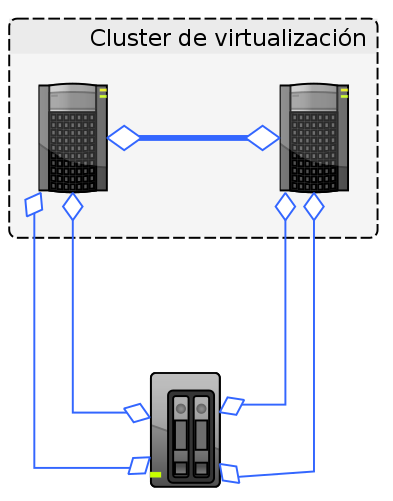
\includegraphics[scale=0.5]{cluster-anterior}
\end{figure}
\par
Como se puede apreciar en el diagrama, cada servidor del cluster se conecta a la cabina por dos conexiones de fibra óptica. Estas conexiones permiten asegurar que siempre haya acceso desde el servidor. Sin embargo, no se tiene acceso a toda la cabina, sino al volumen asignado para almacenar y servir las máquinas virtuales. Por otra parte, algunas maquinas virtuales necesitan tener acceso a volúmenes propios que pueden estar en esta cabina o en otra. 
\par
Los servidores del cluster estaban basados en la versión de largo mantenimiento (LTS) del servidor de Ubuntu \cite{ubuntu}. Esto permite que los servidores siempre estén actualizados y no haya agujeros de seguridad.

\section{Nuevos servicios a prestar}
Al intentar adaptarse a la nueva gestión electrónica que se requiere en la administración pública, ha sido necesario incluir nuevos productos para dar estos nuevos servicios. Para ello, es necesario que algunos de los servicios exisitentes pasen a estar interconectados entre ellos como también actualizarse a productos que se ajusten mejor a las necesidades del Consorcio. 
\par
Los nuevos servicios que se incluirán tras el cambio del cluster son:
\begin{itemize}
    \item Gestión de la contabilidad
    \item Gestión de recursos humanos
    \item Portal del ciudadano
    \item Portal de transparencia
\end{itemize}
Todos los servicios, a excepción del Portal de transparencia, requieren de máquinas virtuales muy potentes con lo que el cluster existente no cumple con los requisitos de memoria, cores ni espacio en el volumen de almacenamiento para albergar estas máquinas y las ya existentes. Por otro lado, para el Portal de transparencia aun no se han establecido los requisitos del software por lo que queda pendiente de implementar.
\par
Para los servicios que sí se van a implementar en esta fase, se requiere de 7 máquinas virtuales con las siguientes características:
\begin{itemize}
    \item 2 Máquinas virtuales con:
    \begin{itemize}
        \item RAM 4GB
        \item vCPU: 1
    \end{itemize}
    \item 1 Máquina virtual con:
    \begin{itemize}
        \item RAM 4GB
        \item vCPU: 2
    \end{itemize}
    \item 2 Máquinas virtuales con:
    \begin{itemize}
        \item RAM 16GB
        \item vCPU: 4
    \end{itemize}
    \item 2 Máquinas virtuales con:
    \begin{itemize}
        \item RAM 6GB
        \item vCPU: 2
    \end{itemize}
    
\end{itemize}

Estas máquinas se separan en dos grupos, 6 máquinas con sistema operativo Microsoft Windows Server 2012 y una con una Ubuntu 14.4 LTS.
Como se puede apreciar, son máquinas con unos requerimientos muy altos. Con lo cual, no se pueden crear en el cluster actual debido a la falta de RAM y vCPU. Debido a esto y a otros proyectos que todavía no se han definido sus requisitos de hardware, es necesario implementar el nuevo cluster, el cual, sí dispone de todos los recursos necesarios para los proyectos actuales como para futuros.
\par
A nivel de funcionamiento de estas máquinas virtuales, es necesario que 4 de ellas estén separadas por parejas en los hypervisores para asegurar la alta disponibilidad. Esto es imposible en el cluster actual. Por otra parte, 6 de las 7 máquinas virtuales están basadas en el sistema operativo de Microsoft Windows 2012.
\section{Requisitos de la solución}

Para la nueva solución es necesario definir los requisitos para una completa integración con la infraestructura.
\begin{itemize}
    \item Debe ser compatible con la infraestructura de Cisco UCS, los blades modelo B200M y los Fabric, tanto Interconnect como los Extender.
    \item Es necesario que el almacenamiento sea distribuido por SCSI y compartido entre todos los hypervisores. Por una parte, habrá un almacenamiento desde el cual se servirán las máquinas virtuales y, por otra parte, cada máquina es posible que requiera de un almacenamiento adicional para su uso.
    \item No debe suponer un problema la migración de las máquinas virtuales desde la vieja plataforma a la nueva.
    \item Los nodos Hypervisores deben servir las máquinas en alta disponibilidad. Esto quiere decir que si uno de los nodos cae, el resto asume sus máquinas virtuales y no se interrumpen los servicios prestados por el nodo caído.
    \item Los hypervisores administrarán 7 redes virtuales para que las máquinas virtuales estén ubicadas en la red según convenga.
    \item Capaz de ejecutar las máquinas virtuales que actualmente se están usando y las nuevas.
    \item No debe suponer ninguna inversión. No se dispone de presupuesto para la implementación de una solución para virtualización.
\end{itemize}

\chapter{Resumen de alternativas y criterios de selección}
\section{Criterios de selección}
A la hora de seleccionar la solución adecuada para la infraestructura, es necesario basarse en los requisitos de la solución vistos anteriormente.
\section{Proxmox Virtual Environment}
Proxmox VE 2.1 proporciona un servidor de virtualización basado en KVM y OpenVz

%Sistema Operativo entero
%Uso de dos tecnologias diferentes para la virtualización
%Gestión 
El mayor problema que se plantea con Proxmox es que para las máquinas virtuales Microsoft Windows Server 2012

\section{CloudStack}
\section{OpenStack}
OpenStack esta enfocado en el despliegue rápido de máquinas y bajo petición.

Para implementar la opción de OpenStack es necesario adaptar los diferentes componentes de la que esta compuesta a la infraestructura existente. Para ello sería necesario instalar tanto el Nova y el Neoutron en todos los hypervisores para que cada hypervisor pueda gestionar las redes de manera independiente y no se cree un cuello de botella en un solo nodo. 
\section{VMware vSphere}

Esta solución en la fase de análisis se descarta de inmediato. El motivo de su descarte es el coste de la solución, ya que no se dispone de presupuesto para ello. Es cierto que esta solución es de las mejores, pero su coste imposibilita su implantación.
\section{Xen + Pacemaker + Corosync}

\chapter{Implementación de la solución seleccionada}

\par A lo largo de este capítulo se explicará el proceso que se ha seguido para la instalación y configuración del los hypervisores. Los cuatro hypervisores son idénticos, por lo que se ha seguido el mismo procedimiento en todos los nodos y en la mayoría de los casos se ha realizado simultáneamente en los cuatro. Se informará de las diferencias que existen entre los cuatro nodos.
\par Al tratarse de una infraestructura crítica, es necesario preservar la seguridad de la entidad, los datos expuestos aquí no son reales, pero el procedimiento es veraz y se describe en detalle.
\section{Instalación del sistema operativo}
%Explicar porque se ha escogido Debian y no otra distribución 
El sistema operativo seleccionado como base ha sido GNU/Debian en su versión estable, la cual, se encontraba en un su release Wheezy, versión 7.3. Se ha escogido Debian debido a su largo ciclo de vida para cada release. Es una instalación básica, pero es necesario hacer algunas matizaciones respecto a algunos pasos.
\begin{itemize}
	\item El idioma seleccionada ha sido el inglés para facilitar la depuración de los errores que vayan surgiendo a lo largo de la configuración y mantenimiento del cluster.
	\item Durante la configuración de la red, se escoge la configuración estática ya que son servidores y necesitamos tener una IP fija y conocida por los administradores, a través de ellas, se realizará el resto de la instalación del resto de componentes del cluster de virtualización. A cada hypervisor se le ha asignado las ips \verb|192.168.200.23|, \verb|192.168.200.24|, \verb|192.168.200.25| y \verb|192.168.200.26| de la red de mantenimiento. Como nombres del servidor se han escogido algo trivial como es \verb|hype1|,\verb|hype2|,\verb|hype3| y \verb|hype4|.
	\item Se han preparado los discos duros con dos particiones, una para el sistema raíz y una swap. En este caso no es necesario un espacio especifico para el usuario ya que no existe o solo es simbólico. La mayoría de las acciones que se van a realizar se realizarán con los permisos del superusuario, \textit{root}. El acceso se realiza mediante las claves publicas de los usuarios que administrarán los servidores, con lo cual la contraseña no es usada. No se han usado los volúmenes lógicos (LVM) ya que no se albergará ninguna máquina virtual dentro de los propios nodos, sino en el volumen servido desde la cabina de almacenamiento y  compartido por todos los nodos.
	\item Tras la instalación del sistema base se han escogido algunas aplicaciones, como es el servidor \verb|ssh| para el acceso remoto y las utilidades de sistema básicas.
\end{itemize}
\section{Instalación y configuración del cliente NTP}
%Explicar las ventajas de usar NTP
Este paso se realiza en todos los hypervisores por igual. Con este componente conseguimos que los cuatro servidores estén sincronizados a la misma hora ya que los cuatro apuntan a un servidor interno de ntp.
\begin{verbatim}
    # apt install ntpdate
    # vim /etc/ntp.conf:
    server 192.168.200.1
\end{verbatim}
\par Tras modificar el fichero \verb|/etc/ntp.conf| se reinicia el servicio de ntp.
\begin{verbatim}
	# service ntp restart
\end{verbatim}
\par Este paso es trivial, sin embargo, de una importancia crucial. Los cuatro hypervisores estarán en constante comunicación para conocer el estado de sus compañeros y el de las máquinas virtuales por lo que un desfase en el tiempo puede hacer que un hypervisor este muerto al percibir una respuesta fuera de hora.
\section{Instalación del hypervisor Xen}
%Terminar de explicar que es Xen
Un hypervisor es una plataforma que permite controlar el hardware y dar los recursos como CPU o RAM a las máquinas virtuales. Xen es de tipo 1 o \textit{bare metal} o sobre el metal desnudo, esto quiere decir que el hypervisor se ejecuta directamente sobre el hardware, con lo que el sistema operativo del host no afecta en la virtualización de las máquinas virtuales.
\par Para convertir una instalación básica de Debian en Dom0 (Host), responsable de ejecutar diferentes instancias de sistemas operativos, es necesario seguir la guía\cite{debianxen} proporcionada por el proyecto de Debian en su wiki.
\begin{verbatim}
    # apt install xen-linux-system xen-tools
\end{verbatim}
El paquete \verb|xen-linux-system| esta compuesto por dos paquetes, por una parte el kernel adaptado para Xen y por otra, las herramientas y el systema de virtualización de Xen en si mismo. Este permite controlar el hardware para poder crear instancias de los sistemas operativos. Las herramientas de \verb|xen-tools| nos facilitarán el manejo y la administración de las máquinas virtuales.
\par Una vez que esta instalado todo, es necesario darle prioridad al núcleo adaptado para Xen para que se arranque por defecto y actualizar el grub para que confirmar los cambios.
\begin{verbatim}
    # dpkg-divert --divert /etc/grub.d/08_linux_xen \
    --rename /etc/grub.d/20_linux_xen
    # update-grub
\end{verbatim}

\section{Configuración de la las interfaces y las VLANs}
Para que tanto los \textit{DomU}, las máquinas virtuales, como el switch virtual, \textit{OpenSwitch}, vean las interfaces de red, es necesario que estén levantadas. Para ello, por cada interfaz incluimos en el fichero \verb|/etc/network/interfaces| las siguientes lineas:
\begin{verbatim}
    auto ethX
    iface ethX inet manual
        pre-up ip link set $IFACE up
        pre-down ip link set $IFACE down
\end{verbatim}
Donde \verb|ethX| representa las interfaces entre \verb|eth0| y \verb|eth15|. Todas estas interfaces las usaremos más adelante en los bridges, puentes, dentro la configuración del OpenSwitch.
\par Exactamente hacemos lo mismo con las VLANs que irán a través de los bridges:
\begin{verbatim}
    auto vlanXXX
    iface vlanXXX inet manual
        pre-up ip link set $IFACE up
        pre-down ip link set $IFACE down
\end{verbatim}
Donde \verb|XXX| representan las VLANs de la red interna, salida a GVA,la red VPN, la salida a Internet y la red de la DMZ.
\par
Se puede apreciar que se dispone de dos redes de almacenamiento, esto es debido a que es un punto crítico de la infraestructura y no se puede perder la conexión con la cabina en ningún momento, por lo que si falla una interfaz de la cabina o la de Fabric Interconnect, el sistema seguiría funcionando por la otra interfaz.
\par Otra cosa que hay que destacar de la configuración de las interfaces es que solo las redes de almacenamiento y la de mantenimiento son las únicas a las que se les ha proporcionado una configuración de red:
\begin{verbatim}
auto vlanSTOR1 
iface vlanSTOR1 inet static 
    address 10.0.50.YY 
    netmask 255.255.255.0 

auto vlanSTOR2 
iface vlanSTOR2 inet static 
    address 10.0.51.YY 
    netmask 255.255.255.0 

auto br1 
iface br1 inet static 
    address 192.168.200.YY #IP asignada al hypervisor
    netmask 255.255.255.0 
    network 192.168.200.0 
    broadcast 192.168.200.255 
    gateway 192.168.200.1 
    dns-nameservers 192.168.200.1 192.168.201.182 192.168.201.189 
    dns-search bomberos 
\end{verbatim}
Donde YY corresponde a la terminación de ip de cada uno de los cuatro nodos. Se puede observar que las VLANs de almacenamiento no tienen ni puerta de enlace, ni dirección de difusión, como tampoco servidores DNS. Esto es debido a que no interactúan al Nivel 3 del modelo ISO ya que son conexiones prácticamente directas entre los nodos y la cabina de almacenamiento, a pesar de ser redes virtuales.
\section{Instalación y configuración de Open vSwitch}
\textit{Open vSwitch}\cite{ovs} es un switch virtual que se utiliza en los sistemas de virtualización como sustituto de las \textit{bridge-utils} de GNU/Linux para realizar los puentes en la capa 2 del modelo ISO. Con este switch virtual conseguimos que las máquinas virtuales se puedan comunicar entre ellas dentro del mismo host, como también con el resto de redes de la infraestructura.
Para instalar todos los componentes necesarios de Open vSwitch, ejecutamos el siguiente comando en la consola como \verb|root|: 
\begin{verbatim}
# apt-get install openvswitch-controller openvswitch-brcompat\
openvswitch-switch openvswitch-datapath-source module-assistant
\end{verbatim}
Esto nos instalará el Open vSwitch dividido en varias partes. En primer lugar, \verb|openvswitch-controller| nos instalará la parte responsable de enrutar los paquetes por el mejor camino, sea su destino una máquina física o virtual dentro o fuera del host.El paquete \verb|openvswitch-brcompat| proporciona a Open vSwitch la habilidad de comportarse como un \textit{bridge}, es decir, como puente de red entre segmentos de la misma red. Esto nos permitirá comunicarnos entre las máquinas virtuales que están en la misma red, pero en hosts diferentes. \verb|openvswitch-switch| proporciona las herramientas y los componentes necesarios en el espacio de usuario. El paquete \verb|openvswitch-datapath-source| proporciona el código fuente del módulo del kernel, para la comunicación entre los componentes de \verb|openvswitch-switch| que se encuentran en el espacio de usuario y el espacio del kernel. Para compilar este módulo usaremos el sistema \verb|module-assistant|.
\par
Este será el primer paso, compilar e instalar el nuevo módulo del kernel, para ello, lo hacemos de la siguiente manera:
\begin{verbatim}
# m-a a-i openvswitch-datapath 
\end{verbatim}
A continuación actviamos el modo \textit{bridge} en Open vSwitch cambiamos la opción \verb|BRCOMPAT| a \verb|yes| \verb|/etc/default/openvswitch-switch|.
\par
Una vez que ya tenemos funcionando el switch virtual es hora de configurar los \textit{bridges}, los responsables de la comunicación entre las interfaces virtuales y las físicas. Empezaremos por configurar las dos VLANs que se comunican con la cabina de almacenamiento. Para ello, usamos el comando \verb|ovs-vsctl| que ha sido instalado con el paquete \verb|openvswitch-switch|.
\begin{verbatim}
# ovs-vsctl add-br vlanSTOR1
# ovs-vsctl add-port vlanSTOR1 eth2 
\end{verbatim}
Lo primero es crear el bridge en si mismo, el que verán las máquinas virtuales, y a continuación le enlazamos la interfaz física a este bridge, que es por donde saldrá el tráfico fuera del host. Este procedimiento lo realizamos también con la otra VLAN de almacenamiento, \verb|vlanSTRO2| y la interfaz física, \verb|eth3|.
\par
Para la red de mantenimiento, la llamaremos \verb|mg1| creamos otro bridge de la misma forma que las anteriores, pero no le asignamos una interfaz. En este caso, le creamos un \textit{bonding}, una combinación de interfaces para asegurar la conectividad entre el host y la red.
\begin{verbatim}
# ovs-vsctl add-bond mg1 bond1 eth4 eth5 lacp=active\
  bond-mode=active-backup    
\end{verbatim}
Además le activamos el Protocolo de control de agregado de enlaces (Link Aggregation Control Protocol)\cite{lacp} con la opción \verb|lacp=active|. También indicamos de qué modo queremos que se comporte esta combinación. En nuestro caso, una de las dos interfaces será la activa y la segunda de respaldo mediante \verb|bond-mode=active-backup|.
\par
Como comentamos en la fase anterior, estas tres redes, \verb|vlanSTOR1|, \verb|vlanSTRO2| y \verb|mg1| son las únicas que tienen una configuración de red proporcionada. 
\par
Para el paso siguiente, es necesario levantar las interfaces restantes y la red de mantenimiento. Para ello ejecutamos la siguiente secuencia de comandos:
\begin{verbatim}
# ip link set eth0 up 
# ip link set eth1 up 
# ip link set eth4 up 
# ip link set eth5 up 
# ip link set br1 up 
# ip link set eth6 up 
# ip link set eth7 up 
\end{verbatim}
Una vez levantadas estas interfaces, se crean los bridges para la red interna, que comunica con GVA, la de los parques, la salida a internet, la red para el wifi y  la red de DMZ. Cada red esta representada por una etiqueta de VLAN, correspondiendo respectivamente a cada red las siguientes etiquetas: \verb|vlanLAN|,\verb|vlanGVA|,\verb|vlanP|,\verb|vlanWAN|,\verb|vlanWLAN| y \verb|vlanDMZ|. Las interfaces y los bondings asignados a cada VLAN quedan así:
\begin{itemize}
    \item vlanLAN: eth0 y eth1; bond0
    \item vlanGVA: eth6 y eth7; bond2
    \item vlanP: eth8 y eth9; bond3
    \item vlanWAN: eth10 y eth11; bond4
    \item vlanWLAN: eth12 y eth13; bond4
    \item vlanDMZ: eth14 y eth15; bond5
\end{itemize}
Por cada VLAN se realiza el siguiente procedimiento sustituyendo la VLAN, las interfaces y el bonding asociado.
\begin{verbatim}
# ovs-vsctl add-br vlanLAN1
# ovs-vsctl add-bond vlanLAN1 bond0 eth0 eth1 lacp=active 
# ovs-vsctl set port bond0 other_config:bond-rebalance-interval=10000
\end{verbatim}
Para todas ellas se ha activado el \verb|lacp| como lo hemos hecho con la red de mantenimiento. Además, hemos dejado los dos puertos activos y configurado el balanceo de carga por estas dos interfaces. La carga se rebalanceará cada 10000 ms. 
\par Una vez que ya tenemos todos los bridges configurados solo queda levantar las interfaces y VLANs:
\begin{verbatim}
    # ip link set eth8 up
    # ip link set eth9 up
    # ip link set eth10 up
    # ip link set eth11 up
    # ip link set eth12 up
    # ip link set eth13 up
    # ip link set eth14 up
    # ip link set eth15 up

    # ip link set vlanLAN1 up
    # ip link set vlanDMZ2 up
    # ip link set vlanWLAN6 up
    # ip link set vlanWAN5 up
    # ip link set vlanP up
    # ip link set vlanGVA3 up
\end{verbatim}
Una vez que tenemos todas las interfaces y VLANs levantadas, podemos verificar la configuración con el comando \verb|ovs-vsctl list|. Al realizar las pruebas de balanceo se detecto que existían bucles en algunos switches catalyst de Cisco porque no gestiona bien los bondings activo-activo, por lo que se modificó el modo de funcionamiento de las redes \verb|vlanLAN|, \verb|vlanGVA|, \verb|vlanP|, \verb|vlanWAN|, \verb|vlanWLAN| y \verb|vlanDMZ| para que las interfaces físicas funcionaran en modo activa y respaldo.  Para verificar el estado de los bondings se ha ejecutado el siguiente comando: 
\begin{verbatim}
    # ovs-appctl bond/list
        bond    type            slaves
        bond0   balance-slb     eth0, eth1
        bond4   balance-slb     eth10, eth11
        bond3   balance-slb     eth9, eth8
        bond6   balance-slb     eth15, eth14
        bond5   balance-slb     eth12, eth13
        bond2   balance-slb     eth6, eth7
        bond1   active-backup   eth5, eth4
\end{verbatim}
Se puede apreciar que el único que esta en \verb|active-backup| es el bonding correspondiente a la red de mantenimiento. El resto de los bondings son del tipo \verb|balance-slb| que las interfaces actúan en modo activo-activo e intentan rebalancear la carga en función de la dirección MAC de origen. Este comportamiento los switchs de Cisco de la infraestructura no son capaces de procesar debido a la antigüedad que tienen. Por lo que se tomo la decisión de configurarlo exactamente igual que el bonding de la red de mantenimiento, \verb|active-backup|.
\begin{verbatim}
# ovs-vsctl set port bond0 bond_mod=active-backup lacp=active
# ovs-vsctl set port bond2 bond_mod=active-backup lacp=active
# ovs-vsctl set port bond3 bond_mod=active-backup lacp=active
# ovs-vsctl set port bond4 bond_mod=active-backup lacp=active
# ovs-vsctl set port bond5 bond_mod=active-backup lacp=active
# ovs-vsctl set port bond6 bond_mod=active-backup lacp=active
\end{verbatim}
En todos los casos, hemos dejado activado el \verb|lacp| para la gestión del bonding. Verificamos el nuevo estado de los bondings: 
\begin{verbatim}
    # ovs-appctl bond/list
        bond    type            slaves
        bond0   active-backup   eth1, eth0    
        bond4   active-backup   eth11, eth10  
        bond3   active-backup   eth9, eth8    
        bond6   active-backup   eth15, eth14  
        bond5   active-backup   eth12, eth13  
        bond2   active-backup   eth7, eth6    
        bond1   active-backup   eth5, eth4
\end{verbatim}
Con esto, los switches más antiguos dejarán de crear bucles. Sin embargo, se detecto otro problema, las interfaces no se levantaban al arrancar el nodo. Revisando las posibles causas, se encuentra que es el BUG \#686518\cite{bug} de la versión usada y que no se ha planteado todavía por parte de los desarrolladores una solución para la siguiente. Por otro lado, una solución a este BUG es forzar en el script de inicio  \verb|/etc/init.d/openvswitch-switch| el levantamiento de todas las interfaces. Así quedaría el final de la función de \verb|start| del script de opevswitch-switch:
\begin{verbatim}
        ...
        "$@" || exit $?
        ovs_ctl --protocol=gre enable-protocol
        ifup -a
}
\end{verbatim}
Añadiendo el comando \verb|ifup -a| levantaremos todas las interfaces y las VLANs al terminar el arranque del servicio \verb|openvswitch-switch|.
\section{Instalación del multipath}
El \textit{Device Mapper Multipath}permite establecer diferentes rutas o caminos de entrada y salida entre las cabinas de almacenamiento y los nodos servidores a través de un mismo dispositivo. Estas rutas de I/O son conexiones físicas que pueden incluso estar separadas por switches, controladoras o cables. Multipath agrega las rutas de I/O creando un nuevo dispositivo. En otras palabras, el DM-Multipathing crea un dispositivo dentro del nodo servidor que permitirá acceder a la cabina mediante la agregación de caminos en dicho dispositivo. 
\section{Instalación de Corosync y Pacemaker}


\chapter{Resultados y conclusiones}
%Posibles mejoras
%Posibles lineas de investigación
\chapter{Anexos}
%Ficheros de configuración

%\chapter{Bibliografía}
\nocite{*}
%\printbibliography

\end{document}